\documentclass[10pt, letterpaper]{report}
% !TeX program = xelatex
%==================PREAMBOLO=======================%
\usepackage[utf8]{inputenc}
\usepackage{psvectorian}
\usepackage{pgfplots}
\usepackage[Rejne]{fncychap}
\usepackage[export]{adjustbox}
\usepackage[T1]{fontenc}
\usepackage{lmodern}
\usepackage[shortlabels]{enumitem}
\usepackage{moresize}
\usepackage{graphicx} % Required for inserting images
\usepackage{hyperref}
\usepackage{listings}
\usepackage[table,xcdraw]{xcolor}
\usepackage{amssymb}
\usepackage{amsmath}
\usepackage[italian]{babel}
\usepackage{nicefrac, xfrac}
\usepackage{tikz}
\usepackage{mathrsfs} 
\usepackage{titletoc}
\usepackage{fancyhdr}
\usepackage{psvectorian,lipsum}
\usepackage{fourier-orns}
\usepackage{lipsum}
\usepackage[paper=a4paper,left=25mm,right=25mm,bottom=25mm,top=25mm]{geometry}
\definecolor{light-gray}{gray}{0.95}
\definecolor{cop}{HTML}{f7ecd7}
\definecolor{copAut}{HTML}{ababab}
\definecolor{copAut2}{HTML}{c3c3e6}
\definecolor{purcop}{HTML}{d0d3db}
\definecolor{sapienza}{HTML}{660f1d}
\definecolor{lightSapienza}{HTML}{e3d3d5}
\definecolor{darkgreen}{HTML}{008000}
\definecolor{cartaRiciclata}{HTML}{fcfcf7}
\newcommand{\redText}[1]{\color{red}#1\color{black}}
\newcommand{\code}[1]{\colorbox{light-gray}{\texttt{#1}}}
\newcommand{\codee}[1]{\colorbox{white}{\texttt{#1}}}
\newcommand{\K}{{\mathbb K}}
\newcommand{\notimplies}{%
  \mathrel{{\ooalign{\hidewidth$\not\phantom{=}$\hidewidth\cr$\implies$}}}}
\newcommand{\flowerLine}{ \begin{center}\decofourleft\hphantom{ }\decoone\hphantom{ }\decofourright\hphantom{}\hphantom{aa}
\decofourleft\hphantom{ }\decoone\hphantom{ }\decofourright\hphantom{}\hphantom{aa}
\decofourleft\hphantom{ }\decoone\hphantom{ }\decofourright\hphantom{}\hphantom{aa}
\decofourleft\hphantom{ }\decoone\hphantom{ }\decofourright\hphantom{}\hphantom{aa} 
\decofourleft\hphantom{ }\decoone\hphantom{ }\decofourright\hphantom{}\hphantom{aa}
\decofourleft\hphantom{ }\decoone\hphantom{ }\decofourright\hphantom{}\hphantom{aa}
\decofourleft\hphantom{ }\decoone\hphantom{ }\decofourright\hphantom{}\hphantom{aa}
\decofourleft\hphantom{ }\decoone\hphantom{ }\decofourright\hphantom{}\hphantom{aa}
\decofourleft\hphantom{ }\decoone\hphantom{ }\decofourright\hphantom{}\hphantom{aa}
\end{center}}
\definecolor{g}{RGB}{60, 50, 50}
\newcommand{\textg}[1]{\color{g}{\textbf{#1}}\color{black}}
\newcommand{\teo}[1]{{\large\color{sapienza}\textbf{Teorema #1 :\hphantom{a}}}}
\newcommand{\defi}[1]{{\large\color{sapienza}\textbf{Definizione #1 :\hphantom{a}}}}
\newcommand{\claim}[1]{{\color{sapienza}\textbf{Claim #1 :\hphantom{a}}}}
\newcommand{\lemma}[1]{{\color{sapienza}\textbf{Lemma #1 :\hphantom{a}}}}
\newcommand{\dimo}[1]{{\color{sapienza}\textbf{Dimostrazione #1 :\hphantom{a}}}}
\newcommand{\prop}[1]{{\color{sapienza}\textbf{Proposizione #1 :\hphantom{a}}}}
\newcommand\greybox[1]{%
  \vskip\baselineskip%
  \par\noindent\colorbox{light-gray}{%
    \begin{minipage}{\textwidth}#1\end{minipage}%
  }%
  \vskip\baselineskip%
}
\newcommand\sapbox[1]{%
  \vskip\baselineskip%
  \par\noindent\colorbox{lightSapienza}{%
    \begin{minipage}{\textwidth}#1\end{minipage}%
  }%
  \vskip\baselineskip%
}

\newcommand{\Z}{{\mathbb Z}}
\newcommand{\blank}{{\sqcup}}
\newcommand{\R}{{\mathbb R}}
\newcommand{\N}{{\mathbb N}}
\newcommand{\C}{{\mathbb C}}
\newcommand{\Sn}{{\mathcal S_n}}
\newcommand{\An}{{\mathcal A_n}}
\newcommand{\E}{{\mathcal E}}
\newcommand{\B}{{\mathcal B}}
\newcommand{\mcm}{{\text{mcm}}}
\newcommand{\rg}{{\text{rg}}}
\newcommand{\ve}{{\bar v}}
\newcommand{\spaz}{{\text{\hphantom{aa}}}}
\newcommand{\MCD}{{\text{MCD}}}
\newcommand{\tc}{{\text{ tale che }}}
\newcommand{\supp}{{\text{Supp}}}
\newcommand{\acc}{\\\hphantom{}\\}
\newcommand{\aut}{{\text{Aut}}}
\newcommand{\Span}{{\text{Span}}}
\newcommand{\End}{{\text{End}}}
\newcommand{\cen}{{\text{Centro}}}
\newcommand{\norm}{{\unlhd}}
\newcommand{\ciclS}{{\left \langle }}
\newcommand{\ciclE}{{\right \rangle }}
\newcommand{\boxedMath}[1]{\begin{tabular}{|c|}\hline \texttt{#1} \\ \hline\end{tabular} :}
\newcommand{\shell}[1]{\colorbox{black}{\textcolor{white}{\texttt{#1}}}}
\newcommand{\eqImportante}[1]{\begin{center}\huge\lefthand\hphantom{a}
    \normalsize\texttt{#1}
    \hphantom{aaa}\huge\righthand\end{center}}

\fancyhf{}
\pagestyle{fancy}
\usepackage{pgf-pie}  
\usetikzlibrary{positioning}

\renewcommand{\headrule}{%
\vspace{-8pt}\hrulefill
\raisebox{-2.1pt}{\quad\decothreeleft\decotwo\decothreeright\quad}\hrulefill}

%sta roba serve per il codice C
\definecolor{mGreen}{rgb}{0,0.6,0}
\definecolor{mGray}{rgb}{0.5,0.5,0.5}
\definecolor{mPurple}{rgb}{0.58,0,0.82}
\definecolor{backgroundColour}{rgb}{0.95,0.95,0.92}

\lstdefinestyle{CStyle}{
    backgroundcolor=\color{backgroundColour},   
    commentstyle=\color{mGreen},
    keywordstyle=\color{magenta},
    numberstyle=\tiny\color{mGray},
    stringstyle=\color{mPurple},
    basicstyle=\footnotesize,
    breakatwhitespace=false,         
    breaklines=true,                 
    captionpos=b,                    
    keepspaces=true,                 
    numbers=left,                    
    numbersep=5pt,                  
    showspaces=false,                
    showstringspaces=false,
    showtabs=false,                  
    tabsize=2,
    language=C
}
\lstdefinestyle{CppStyle}{
    backgroundcolor=\color{backgroundColour},   
    commentstyle=\color{mGreen}\ttfamily,
    morecomment=[l][\color{magenta}]{\#}
    keywordstyle=\color{blue}\ttfamily,
    numberstyle=\tiny\color{mGray},
    stringstyle=\color{red}\ttfamily,
    basicstyle=\ttfamily,
    breakatwhitespace=false,         
    breaklines=true,                 
    captionpos=b,                    
    keepspaces=true,                 
    numbers=left,                    
    numbersep=5pt,                  
    showspaces=false,                
    showstringspaces=false,
    showtabs=false,                  
    tabsize=2,
    language=C
}
\lstset{language=C++,
                basicstyle=\ttfamily,
                keywordstyle=\color{blue}\ttfamily,
                stringstyle=\color{red}\ttfamily,
                commentstyle=\color{green}\ttfamily,
                morecomment=[l][\color{magenta}]{\#}
}
%fine roba che serve per il codice C
\usepackage{minted}
 %TOGLI COMMENTO SE USI XELATEX
%\usepackage{fontspec}
\title{\jobname} %========TITOLO========%
\author{Marco Casu}
\date{\vspace{-5ex}}
\begin{document}

%==================COPERTINA=======================%
\begin{titlepage}
    \pagecolor{cartaRiciclata}
\begin{center}
    %TOGLI COMMENTO SE USI XELATEX
   %\setmainfont{Palace Script MT}
   \HUGE Marco Casu\acc
    %\setmainfont{Grand Casino}
     %TOGLI COMMENTO SE USI XELATEX
    %\setmainfont{h Halfroad}
    \HUGE \decothreeleft\hphantom{ }{\fontsize{48}{50}\selectfont \jobname}\hphantom{ }\decothreeright
     %TOGLI COMMENTO SE USI XELATEX
   % \setmainfont{Times New Roman}
\end{center}
\thispagestyle{empty}
\begin{figure}[h]
    \centering{
        %l'immagine deve avere una risoluzione 2048x2048
        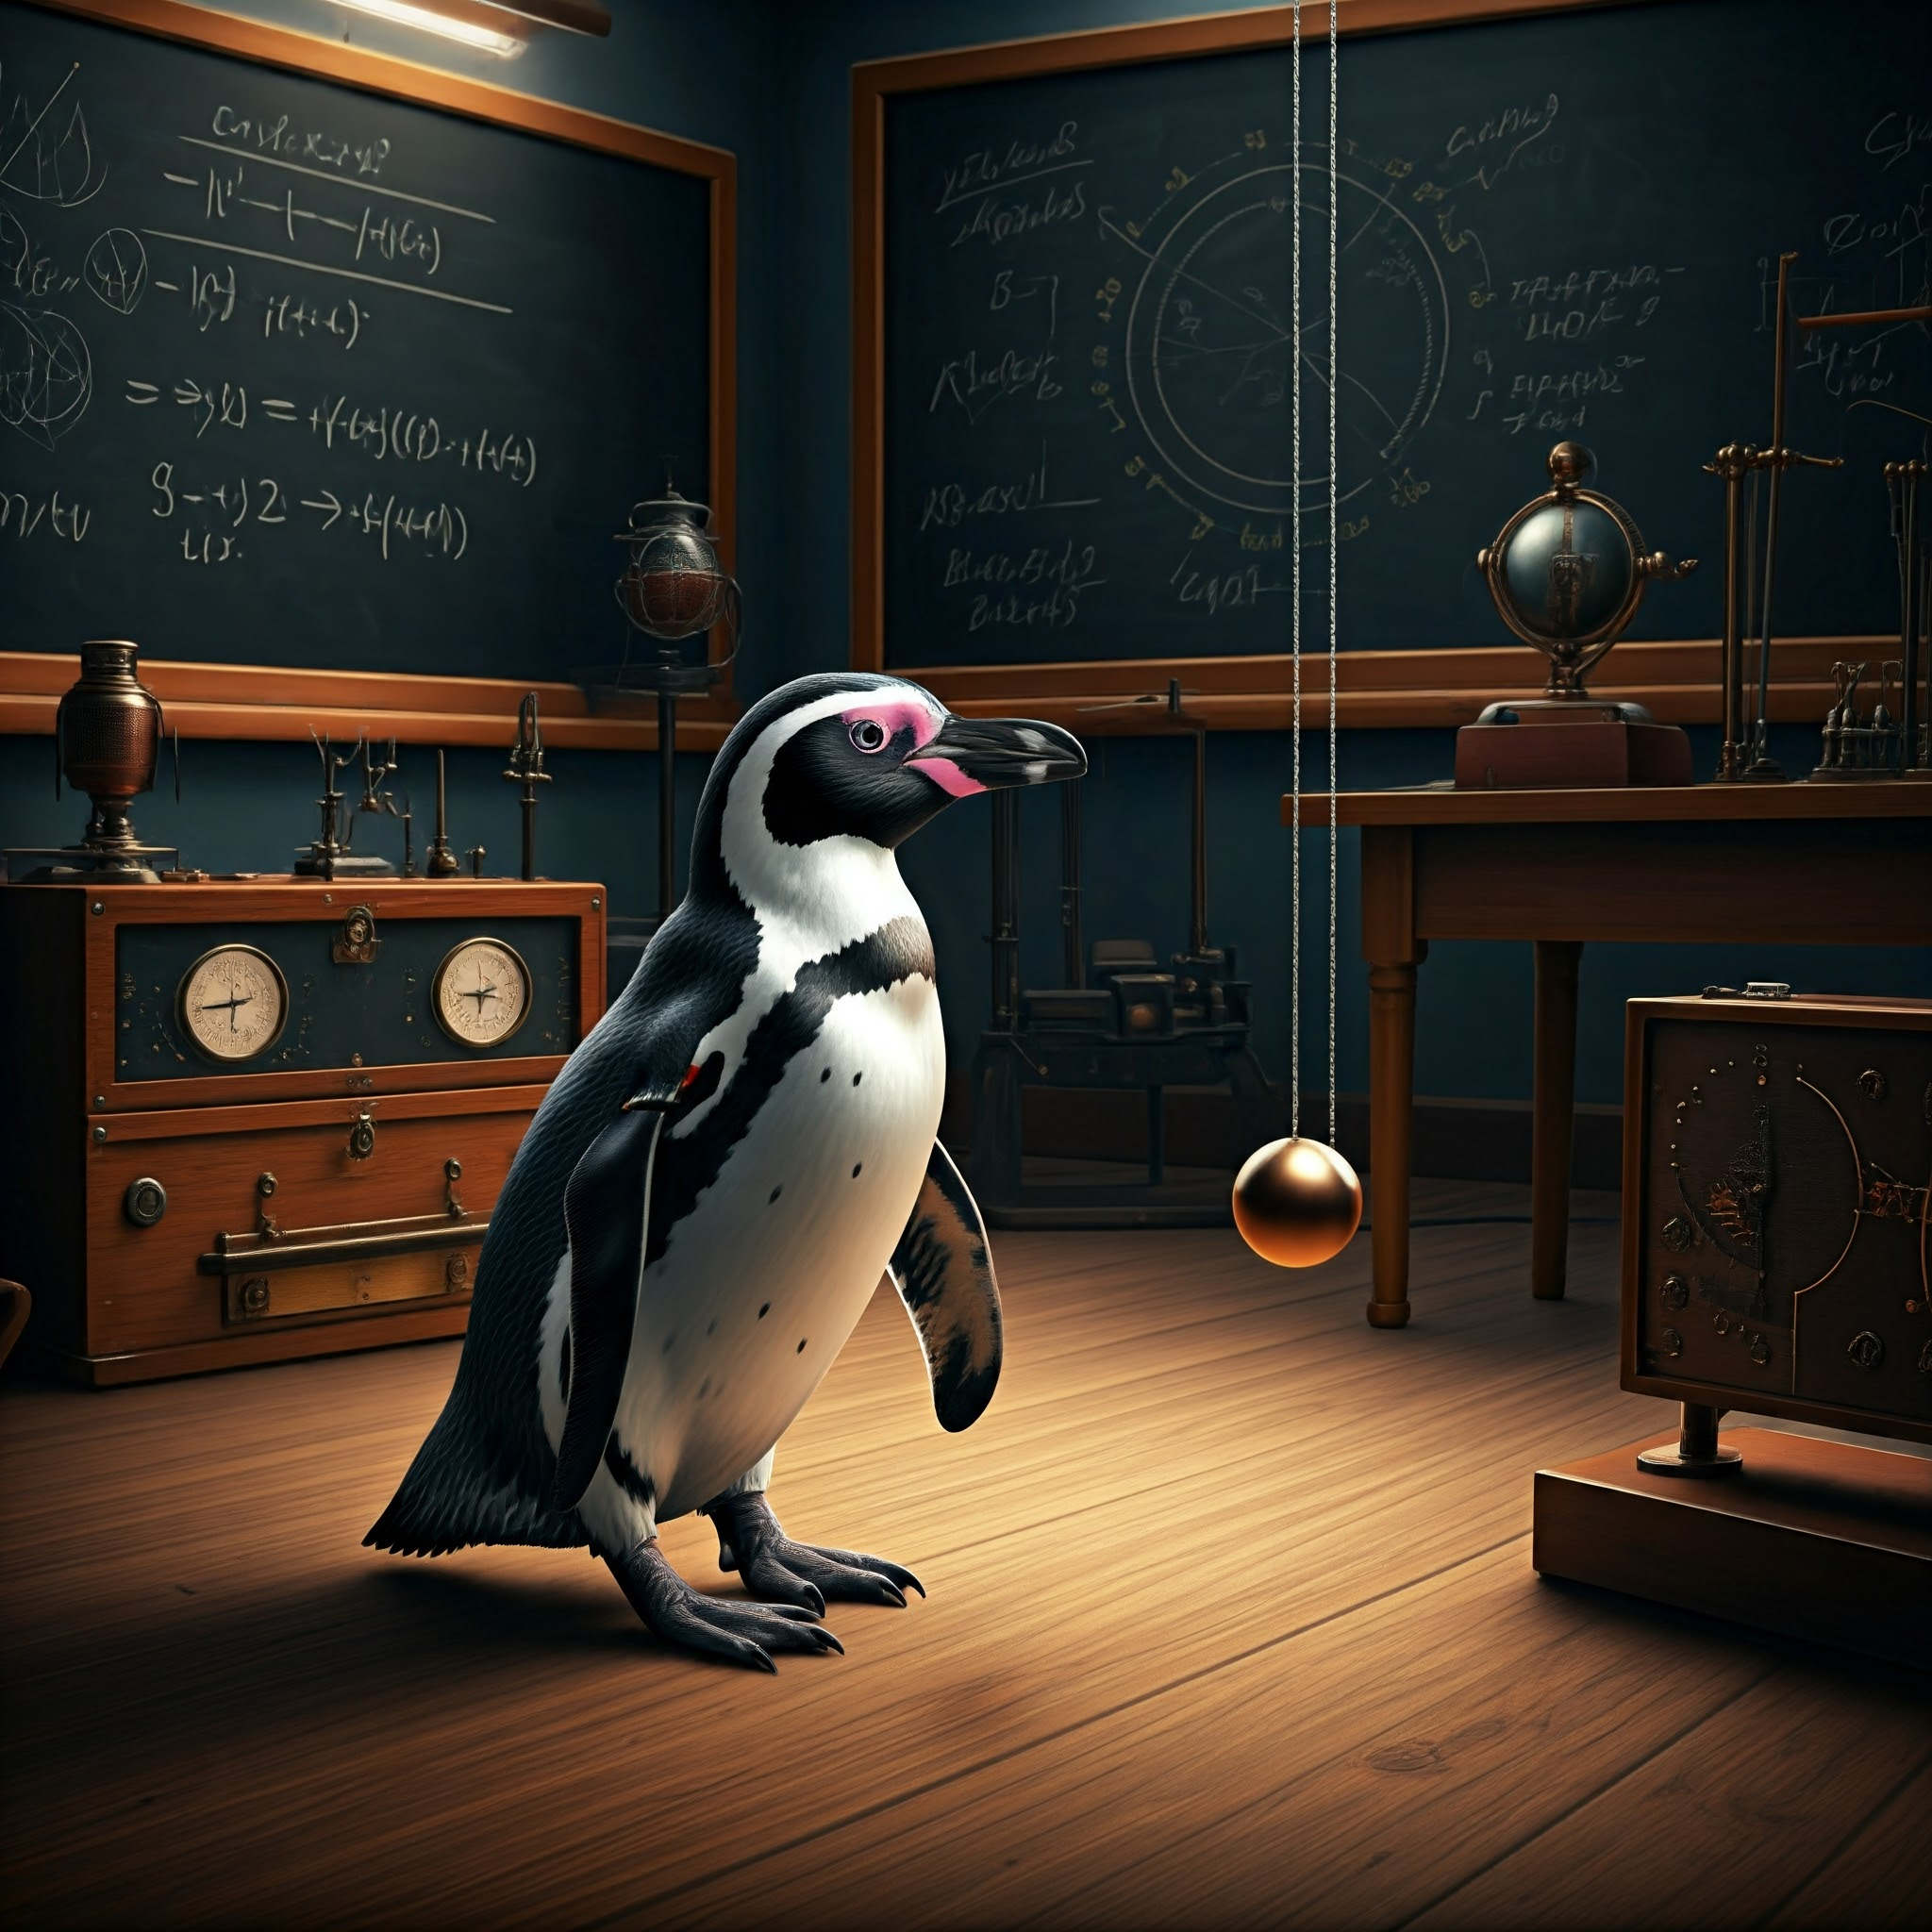
\includegraphics[width=1\textwidth ]{images/copertina.jpg}
    }
\end{figure}
\vfill 
\centering 
\includegraphics[width=0.4\textwidth ]{../../preamble/Stemma_sapienza.png} \acc
\centering \Large \color{sapienza}Facoltà di Ingegneria dell'Informazione,
Informatica e Statistica\\
Dipartimento di Informatica
\end{titlepage}

%===================FINE COPERTINA======================%
\newpage
\pagecolor{cartaRiciclata}%\setmainfont{Algerian}
Questo documento è distribuito sotto la licenza 
\color{blue}\href{https://www.gnu.org/licenses/fdl-1.3.txt}{GNU}\color{black},  
è un resoconto degli appunti (eventualmente integrati con libri di testo) tratti dalle lezioni del corso di \jobname
\hphantom{a}per la laurea 
triennale in Informatica. Se dovessi notare errori, ti prego di segnalarmeli.
\newpage %\setmainfont{Times New Roman}
\normalsize
\tableofcontents 
\newpage

%==================FOOTER e HEADER=======================%
\fancyhf{}
\fancyhead[L]{\nouppercase{\leftmark}}
\fancyhead[R]{Sezione \thesection}
\fancyfoot[C]{\thepage}
\fancyfoot[L]{Appunti di \jobname}
\fancyfoot[R]{ Marco Casu}
%\fancyfoot[R]{\setmainfont{Palace Script MT}\huge Marco Casu \setmainfont{Times New Roman}}
%==================FOOTER e HEADER=======================%

%Ricorda del comando \flowerLine per separare le sottosezioni. Le sezioni si separano nelle diverse pagine

%==================INIZIO======================%

\chapter{Introduzione}
\section{Il metodo scientifico}
La nascita del metodo scientifico è dovuta a Galileo Galilei, se i filosofi greci stabilivano 
leggi empiriche senza necessariamente dimostrarle, Galileo introdusse una verifica sperimentale 
a quelle che erano le sue digressioni.\acc 
Un \textbf{esperimento}, è una verifica sperimentale delle ipotesi, utile a ricavare valori 
numerici oggettivi per le misure delle grandezze fisiche. L'avvento del cannocchiale permise un 
osservazione più accurata dei corpi celesti, questi che venivano creduti perfetti, si rivelarono 
per quello che sono, la Luna con i suoi accavallamenti e "mari", mostrava una 
conformazione della sua crosta tutto fuorché perfetta.
\begin{figure}[h!]
    \centering
    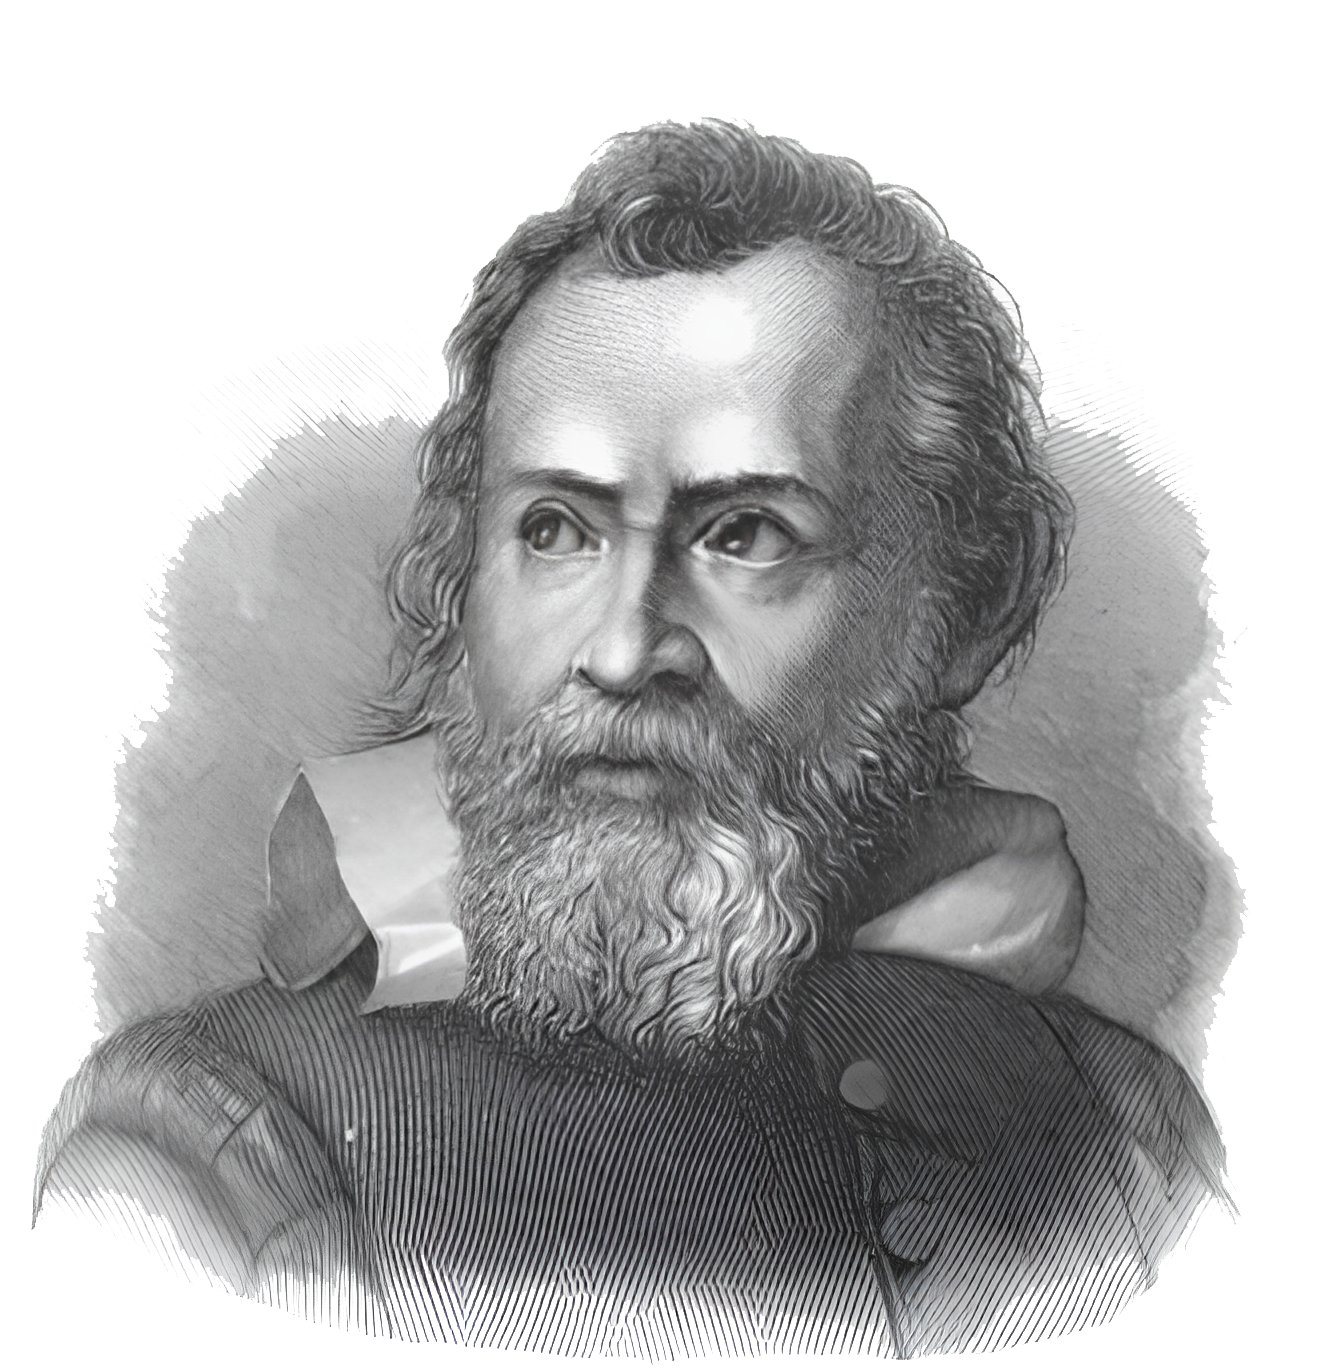
\includegraphics[width=140pt]{images/Galileo2.png}
    \caption{ Galileo Galilei}
    \label{fig:Galileo}
\end{figure}
Oltre al già citato cannocchiale, erano necessari ulteriori strumenti per le osservazioni dei 
corpi celesti, era necessario misurare in maniera precisa ed affidabile lo scorrere del tempo. 
Misurare il tempo vuol dire confrontare due eventi, ad esempio, il sorgere del sole con il movimento 
periodico riferito ad un misuratore (come l'orologio).\acc 
Galileo per le sue misure realizzò un orologio ad acqua, utilizzando un recipiente nella quale 
riporre un piccolo foro sul fondo, in modo tale che l'acqua cadesse a gocce a velocità costante, 
così facendo, lo scorrere del tempo era proporzionale al volume dell'acqua perso dall recipiente.\acc 
Una \textbf{grandezza fisica} è un entità alla quale si attribuisce una specifica definizione, utilizzabile 
per descrivere un fenomeno fisico, per tali entità devono valere i criteri di uguaglianza e 
sommabilità.\acc 
Uno degli argomenti su cui si soffermò Galileo fu il \textit{moto dei gravi}, in particolare 
il moto dei corpi in caduta libera. Secondo la fisica aristotelica del tempo, un corpo 
tanto più pesante era, tanto più rapidamente cadeva. \acc 
Galileo fu critico nei riguardi di questa visione, osservò che in realtà, ogni corpo 
cade verso il suolo con la stessa accelerazione, il motivo per il quale una piuma cade 
più rapidamente di una sfera di piombo non riguarda la loro massa, bensì la resistenza dell'aria 
nei confronti del loro materiale e della loro forma. Trovò inoltre che la distanza percorsa 
durante la caduta di un oggetto è proporzionale al quadrato del tempo impiegato per percorrerla.\acc 
Galileo con un esperimento riguardante i piani osservò il seguente fatto : 
    \textit{se si lascia scivolare un corpo su un piano inclinato ad altezza $h$ per poi 
    farlo risalire su un altro piano inclinato, questo tendeva a risalire fino alla 
    stessa altezza $h$}.
    \begin{figure}[h!]
        \centering
        \includegraphics[width=500pt]{images/cadutaGraveBW.eps}
        \caption{ caduta sul piano inclinato}
        \label{fig:caduta}
    \end{figure}\acc
Inoltre, notò che questo fenomeno non è condizionato dal seno dell'angolo del piano, bensì 
esclusivamente dall'altezza.
\begin{figure}[h!]
    \centering
    \includegraphics[width=500pt]{images/cadutaGrave2BW.eps}
    \caption{ inclinazioni differenti}
    \label{fig:caduta2}
\end{figure}\acc
Per osservare tale risultato dovette ridurre le azioni spurie dell'attrito dell'aria. Più 
il percorso era liscio, più l'attrito risultava debole, e più il corpo tendeva ad 
avvicinarsi all'altezza originale $h$. Con tale ragionamento ipotizzò che se l'attrito dovesse 
essere stato nullo, allora il corpo sarebbe tornato precisamente all'altezza $h$.\acc 
Dato questo per vero, riducendo il valore dell'angolo sarebbe stato possibile far percorrere 
al corpo una distanza maggiore. Se il secondo piano avesse avuto inclinazione nulla, allora 
il grave avrebbe continuato a muoversi in avanti a velocità costante.\begin{figure}[h!]
    \centering
    \includegraphics[width=330pt]{images/cadutaGrave3BW.eps}
    \caption{ inclinazione nulla}
    \label{fig:caduta3}
\end{figure}\acc
Tale principio è noto come \textbf{legge d'Inerzia}, eliminando gli attriti, lo stato di moto naturale inalterato di
un corpo è quello di moto rettilineo uniforme (a velocità costante) indefinitamente.\acc 
Essendo la scienza sempre stata impiegata anche in ambito bellico, Galileo studiò il moto dei 
proiettili, che fino a quel momento si credeva fosse costantemente orizzontale, fino al momento in 
cui il proiettile perdeva il suo "impeto" cadendo a terra. Egli si rese conto che 
i proiettili sono soggetti sia alla forza impressa dal colpo (orizzontale), sia a quella verticale 
impressa verso il basso.\acc 
La forza impressa dal colpo gli da una velocità costante, in quanto non è soggetto ad ulteriori 
accellerazioni orizzontalmente, quella verticale invece provoca un moto uniformemente accellerato, 
la distanza 
percorsa in verticale è proporzionale al 
quadrato del tempo impiegato a percorrerla, la combinazione dei due moti risulta in un arco 
di parabola.
\begin{center}
	\begin{tabular}{>{\centering\arraybackslash}m{3in}>{\centering\arraybackslash}m{3in}}
		\begin{tikzpicture}[scale=0.9, transform shape]
		\begin{axis}[
		ymin=-6,
		ymax = 6,
		xmin=-6,
		xmax = 6,
		axis lines = center,
		xtick distance=2, ytick distance=2,
		grid style=dashed,
		ymajorgrids=true,
		xmajorgrids=true,
		xlabel = \(\),
		ylabel = {\(\)},
		]
		%Below the red parabola is defined
		\addplot [
		domain=-6:6,
		samples=20,
		color=blue,
		]
		{-(1/5)*(x^2)};
		\addlegendentry{\(y=-\nicefrac{1}{5}\cdot x^2\)}
		\end{axis}
		\end{tikzpicture} &   
		Galileo, chiamò $x$ la direzione orizzontale, ed $y$ quella verticale, partendo da 
		$(x,y)=(0,0)$, e sapendo che lo spazio percorso in $x$ è proporzionale ale tempo, mentre 
		quello percorso in $y$ è proporzionale al quadrato del tempo, si ha 
		$$ x=a\cdot t\;\;\;\;\;\;\;\;\;\;\;\; y = b\cdot t^2$$
		Con alcuni passaggi algebrici si trova esattamente la nota equazione della parabola
		$$ y=\frac{b}{a^2}\cdot x^2$$
		\\
	\end{tabular}
\end{center}
\flowerLine 
\section{Spostamento, Velocità e Grandezze Fisiche}
Il \textbf{moto}, è uno dei fenomeni fisici più classici, che necessita 
di una definizione e rappresentazione formale, è il cambiamento 
di una posizione rispetto al tempo.\acc 
Un classico esempio di sistema di riferimento è il piano cartesiano, 
in cui un punto nello spazio, è identificato da tre coordinate 
$$ (x(t),y(t),z(t))$$
In funzione del tempo $t$. Può essere rappresentato anche da 
un vettore posizione $\bar r(t)$, descritto dalla lunghezza 
e dagli angoli rispetto gli assi del piano e la proiezione 
delle sue componenti, nel caso bi-dimensionale, sia $r$ il modulo 
del vettore $\bar r$ :
\begin{figure}[h!]
    \centering
    \includegraphics[width=100pt]{images/vecAngolo.eps}
    \caption{ $\bar r = (r,\theta)$}
    \label{fig:vecAng}
\end{figure}\acc 
Risulta possibile passare dalle coordinate cartesiane a quelle descritte 
con l'angolo tramite le seguenti trasformazioni 
$$\begin{cases}
    r\cos(\theta)=x\\ r\sin(\theta)=y
\end{cases} $$
Inoltre 
$$r^2(\cos^2(\theta)+\sin^2(\theta))=x^2+y^2$$
$$r=\sqrt{x^2+y^2}\ \ \ \ \ \ \ \ \theta = \arctan(\nicefrac{y}{x})$$
Le componenti di $\bar r$ dipendono dal sistema di riferimento.
Posso definire uno \textit{spostamento nel tempo}, tramite il vettore 
$\bar r$ in un istante $t$, ed il medesimo vettore in un istante 
$t+\Delta t$, dove $\Delta t$ rappresenta una variazione temporale. 
Una volta definiti i vettori $\bar r (t)$ e $\bar r (t+\Delta t)$,
 si definisce il \textbf{vettore spostamento} come la loro 
 differenza algebrica, ossia $\Delta \bar r = \bar r (t+\Delta t)-\bar r (t)$.
 \begin{center}
    \centering
    \begin{minipage}{.5\textwidth}
      \centering
      \includegraphics[width=.5\linewidth]{images/spostamento.eps}
    \end{minipage}%
    \begin{minipage}{.5\textwidth}
      \centering
      \includegraphics[width=.5\linewidth]{images/vecSpostamento.eps}
    \end{minipage}
\end{center}
Si vogliono rappresentare i vettori in maniera più formale, rispetto 
che alla classica notazione $\bar v = (x,y,z)$. Si fa uso dei versori 
$$ \bar i = (1,0,0)\ \ \ \
\bar j = (0,1,0)\ \ \ \  
\bar k = (0,0,1) $$
per definire un vettore come somma dei versori scalati con appositi 
 coefficienti, che rappresentano le componenti del vettore : 
 $$ \bar v = (x,y,z) = x\bar i+y\bar j+z \bar k $$
 Ogni componente della somma è la proiezione del vettore su uno dei 
 tre assi. Si osservi come il vettore spostamente non dipende dal sistema di riferimento.\acc 
 Il vettore spostamento $\Delta \bar r$ varia a sua volta nel tempo, 
 descrivendo quindi il moto di un punto, la \textbf{velocità media} di tale 
 spostamento si definisce tramite il rapporto incrementale 
 $$ 
 \frac{\Delta \bar r (t)}{\Delta t}=\frac{\bar r(t+\Delta t)-\bar r(t)}{\Delta t}
 $$
Si può definire anche la velocità media scalare, se lo spostamento avviene 
su un percorso già definito, e non è necessaria informazione sulla 
direzione, è possibile rappresentarlo con uno scalare 
$s(t)$, e $\dfrac{\Delta s}{\Delta t}$ rappresenta la velocità media 
scalare.\acc 
La velocità media non è molto precisa come informazione, in quanto 
non descrive il moto di un corpo (la sua traiettoria) a pieno, 
si vuole quindi dare una misura di una velocità \textit{istantanea}, 
si fa quindi tendere a zero la differenza di tempo : 
$$
\lim_{\Delta t\rightarrow 0} \frac{\Delta \bar r (t)}{\Delta t}=
\lim_{\Delta t\rightarrow 0} \frac{\bar r(t+\Delta t)-\bar r(t)}{\Delta t}
$$
Tale grandezza si denota $\dfrac{d\bar r}{d t}$, è la derivata 
dello spostamento rispetto al tempo, verrà nominata semplicemente  
\textbf{velocità}, e denotata $\bar v$,  rappresenta lo spostamento istantaneo ed è 
tangente alla curva dello spostamento. Si definisce anche la 
velocità scalare  $\dfrac{d s}{d t}$, ed è il modulo della 
velocità.\acc 
Una volta definite delle quantità come spostamento e velocità, è necessario 
definire delle \textit{grandezze fisiche} ed introdurre delle 
\textit{unità di misura}. Il vettore $\bar r$ ha le dimensioni di una lunghezza, la dimensione 
lunghezza $[l]$ è espressa in metri $m$, il sistema internazionale definisce  
$$ (m,kg,s)=\text{ (metri, kilogrammi, secondi)}$$
La dimensione del tempo $[t]$ è espressa in secondi $s$. Esistono alcune grandezze 
dette adimensionali, un esempio sono gli angoli, misurati in gradi o radianti.
\acc 
La velocità, è una grandezza derivata, essendo un rapporto fra lo spostamento ed il tempo, 
si misura in metri al secondo : $\nicefrac{m}{s}$, rappresenta, appunto la distanza in 
metri percorsa in 1 secondo. Le grandezze possono essere convertite, ad esempio, considerando 
i kilometri - orari si ha che 
$$ 1\nicefrac{m}{s}= 
\frac{10^{-3}}{\nicefrac{1}{3600}}\nicefrac{km}{h}= 
10^{-3}\cdot 3600 \nicefrac{km}{h}=3.6\nicefrac{km}{h}$$
Introduciamo adesso il concetto di \textbf{differenziale}, si consideri una generica funzione 
$f(x)$ in un punto $x_0$, ed il suo rapporto incrementale per una variazione $d x$.
\begin{center}
	\begin{tabular}{>{\centering\arraybackslash}m{3in}>{\centering\arraybackslash}m{3in}}
		\includegraphics[width=.8\linewidth]{images/differenziale1.eps} & Il segmento denotato \color{blue}$\Delta f(x)$ \color{black} rappresenta l'incremento 
        effettivo della funzione, e vale $f(x_0+d x)-f(x_0)$.
		\\
	\end{tabular}
\end{center}
Definisco ora il \textbf{differenziale} 
di $f$ come una  \textbf{linearizzazione} della funzione, ossia, si considera nel punto $x_0$ una 
retta tangente alla curva di $f$.
\begin{center}
	\begin{tabular}{>{\centering\arraybackslash}m{3in}>{\centering\arraybackslash}m{3in}}
		\includegraphics[width=.8\linewidth]{images/differenziale2.eps} &Il differenziale \color{darkgreen} $df$ \color{black}da una stima dell'incremento, considerando una funzione lineare (in questo 
        caso bidimensionale, una retta).
		\\
	\end{tabular}
\end{center}
Denotando con $f'$ la derivata di $f$ si ha
$$ df=f'\cdot dx$$
$$ \frac{df}{dx}=f'$$
Le funzioni lineari sono più semplici di quelle non lineari, il punto di tale differenziale 
è che, quando l'incremento $d x$ tende a zero, l'incremento effettivo della funzione 
e l'incremento "stimato" dato dal differenziale tendono allo stesso valore. $$ 
\lim_{d x\rightarrow 0 }f(x_0+dx)=f(x_0)+f'(x_0)\cdot dx
$$
\chapter{Cinematica}
Si è introdotto il vettore spostamento $\delta \bar r$, con la sua relativa formulazione infinitesima 
di velocità $\bar v$, come derivata del vettore posizione $\bar r$. 
Un'altra grandezza fondamentale nello studio del moto dei corpi è la variazione della velocità, definita 
come il limite del rapporto incrementale di quest'ultima rispetto al tempo. 
Tale grandezza prende il nome di \textbf{accelerazione}
$$ \frac{d\bar v}{d t} = \bar a $$
L'accelerazione $\bar a$, o $a$ se riferita ad una grandezza scalare, si misura in 
$\nicefrac{m}{s^2}$, di cui l'unità, indica che ad ogni secondo, la velocità aumenta 
di $1 \nicefrac{m}{s}$, ovviamente anche'essa può dipendere dal tempo. 
$$\bar a=\frac{d\bar v}{dt}=\frac{d^2\bar r}{dt^2}$$
Si consideri adesso lo spostamento in forma scalare $s(t)$, definito su una traiettoria 
curvilinea già definita
\begin{center}
    \begin{figure}[h!]
        \centering
        \includegraphics[width=0.4\textwidth]{images/accScal.eps}
        \caption{velocità scalare}
        \label{fig:velScal}
    \end{figure} 
\end{center}
Di quest'ultima ne voglio ricavare la sua versione vettoriale, sia $\bar\tau(t)$ il versore 
tangente alla curva prestabilita, nell'immagine \ref{fig:velScal}, evidenziato in blu. 
Si avrà che la velocità vettoriale sarà 
$$ \bar v(t)=\dot{s}(t)\cdot \bar\tau(t)$$
Appunto sulla notazione :  $\dot{s}$ è la derivata prima di $s$. 
$\ddot{s}$ è la derivata seconda di $s$. A questo punto è possibile riscrivere 
l'accelerazione nella seguente forma :
$$
\bar a = \dfrac{d}{dt}\bar v(t)=\ddot{s}(t)\cdot \bar\tau(t)+\dot{s}(t)\cdot\dot{\bar\tau}(t)
$$
Si è quindi divisa l'accelerazione in due componenti distinte, la componente 
$\ddot{s}(t)\cdot \bar\tau(t)$ è nota come \textbf{accelerazione tangenziale} e rappresenta 
la variazione nel tempo del modulo della velocità. L'altra componente, verrà ripresa in seguito, 
ha a che fare con la curvatura della traiettoria.\acc 
\section{I Moti}
\subsection{Rettilineo Uniforme} 
Il moto rettilineo uniforme, secondo la legge d'Inerzia, descrive il moto naturale degli 
oggetti quando non sono soggetti a forze. Tale moto è contraddistinto dal fatto che 
l'accelerazione sia nulla, e la velocità costante, (per semplicità, verranno trattate 
le grandezze in forma scalare).
$$\frac{dv}{dt}=0\implies v = v_0 \text{ costante }$$
Si può ricavare facilmente l'equazione dello spostamento $r$ in un 
lasso di tempo che va da $t_0$ fissato, ad un $t$ generico
$$ \frac{dr}{dt}=v=v_0\implies dr=vd_0t\implies\int_{r(t_0)}^{r(t)}dr=\int_{t_0}^tv_0dt $$
$$\int_{t_0}^tv_0dt=v_0\int_{t_0}^tdt=v_0(t-t_0) $$
Si ha che  
$$ r(t)=r(t_0)+v_0(t-t_0)$$
L'equazione che descrive il moto rettilineo uniforme è lineare
\begin{center}
    \begin{tikzpicture}[scale=0.6, transform shape]
        \begin{axis}[
        ymin=0,
        ymax = 3,
        xmin=0,
        xmax = 3,
        axis lines = left,
        xtick distance=0.5, ytick distance=0.5,
        grid style=dashed,
        ymajorgrids=true,
        xmajorgrids=true,
        xlabel = \(t\),
        ylabel = {\(r(t)\)},
        ]
        %Below the red parabola is defined
        \addplot [
        domain=0:3,
        samples=20,
        color=blue,
        ]
        {x};
        \end{axis}
    \end{tikzpicture}
\end{center} 
\subsection{Uniformemente Accelerato}
La caratteristica del moto uniformemente accelerato è quella di avere un accelerazione costante 
$a = a_0 $, si avrà che 
$$ \frac{dv}{dt}=a_0\implies dv =a_0dt\implies \int_{v(t_0)}^{v(t)}dv=\int_{t_0}^tadt\implies$$
$$v(t)=v(t_0)+a_0(t-t_0) $$
Per semplicità, si definisce $v_0=v(t_0)$ la velocità iniziale. A questo punto, avendo nota l'equazione 
della velocità, si ricava la legge oraria, sia $x_0=x(x)$ la posizione iniziale 
$$ \frac{dx}{dt}=v\implies \int_{x_0}^{x(t)}dx=\int_{t_0}^t vdt = \int_{t_0}^tv_0+a_0(t-t_0)dt= 
v_0\int_{t_0}^tdt+a_0\int_{t_0}^t(t-t_0)dt$$
Considero $t'=t-t_0\implies dt'=dt$ 
$$ v_0\int_{t_0}^tdt+a_0\int_{t_0}^t(t-t_0)dt= 
v_0\int_{t_0}^tdt+a_0\int_{0}^{t-t_0}t'dt'=v_0(t-t_0)+\Big[\dfrac{1}{2}a_0t'\Big]_0^{t-t_0}$$
La soluzione oraria è quindi 
$$ x(t)=x_0+v_0\cdot (t-t_0)+\frac{1}{2}a_0\cdot (t-t_0)^2$$
Essa risulta essere l'equazione della parabola, nel caso più semplice in cui la posizione 
iniziale è 0, ed il tempo iniziale pure, si ha  
$$ x(t)=\dfrac{1}{2}a_0t$$
lo spazio percorso è proporzionale al tempo al 
quadrato.
\subsection{Caduta dei Gravi}
La caduta degli oggetti verso il suolo è descritta dal moto uniformemente 
        accelerato. Ogni oggetto nel campo gravitazionale terrestre, all'altezza del mare, subisce un 
        accelerazione di gravità pari a 
        $$ g\simeq 9.81 \nicefrac{m}{s^2}$$ 
        diretta verso il centro della terra. 
\begin{center}
	\begin{tabular}{>{\centering\arraybackslash}m{3in}>{\centering\arraybackslash}m{3in}}
        \includegraphics[width=0.35\textwidth]{images/oggettoLasciatoCadere.eps} & Definiamo un sistema di riferimento in cui il suolo 
        rappresenta lo zero, ed un corpo viene lasciato cadere da un altezza $h$. Per semplicità, 
        il tempo iniziale $t_0$ è uguale a $0$.
		\\
	\end{tabular}
\end{center}
La legge orario che descrive la posizione $y$ dell'oggetto è la segunete 
$$ \begin{cases}
    y(t)=h-\frac{1}{2}gt^2 \\ 
    v(t)=\dfrac{dy}{dt}=-gt
\end{cases}$$
È possibile calcolare l'istante $t^*$ in cui l'oggetto toccherà il suolo : 
\begin{eqnarray} y(t^*)=0\implies h-\frac{1}{2}g{t^*}^2 =0 \\ 
     h=\frac{1}{2}g{t^*}^2 \\ 
     2\frac{h}{g}={t^*}^2 \\ 
     t^*=\sqrt{2\frac{h}{g}}
\end{eqnarray}
\begin{center}
	\begin{tabular}{>{\centering\arraybackslash}m{3in}>{\centering\arraybackslash}m{3in}}
        \includegraphics[width=0.35\textwidth]{images/graveCaduta2.eps} & Se l'oggetto venisse inizialmente lanciato verso l'alto, si avrebbe una velocità iniziale 
        $v_0$ diversa da zero. La forza di gravità agirà sulla velocità dell'oggetto, facendola diminuire fino a farla 
        diventare negativa, facendolo ricadere verso il suolo.
		\\
	\end{tabular}
\end{center}
L'equazione oraria sarebbe$$ \begin{cases}
    y(t)=h+v_0t-\frac{1}{2}gt^2 \\ 
    v(t)=\dfrac{dy}{dt}=v_0-gt
\end{cases}$$
È possibile trovare il punto più alto raggiunto dal grave, esso sarà il punto in cui la velocità 
passerà da essere positiva (l'oggetto si allontana dal suolo) ad essere negativa (l'oggetto si avvicina al suolo), 
raggiungerà quindi il punto più alto nell'istante $t^*$ in cui la velocità è nulla. 
$$ v(t^*)=0\implies v_0-gt^* = 0 \implies t^*=\frac{v_0}{g}$$
La quota massima raggiunta sarà quindi 
\begin{eqnarray}
    t(\nicefrac{v_0}{g}) = h+v_0\nicefrac{v_0}{g}-\frac{1}{2}g(\nicefrac{v_0}{g})^2 =\\ 
    h+\frac{v_0^2}{g}-\frac{v_0}{2g} = \\ 
    h+\frac{1}{2}\frac{v_0^2}{g}
\end{eqnarray}
È possibile riscrivere l'equazione del moto uniformemente accelerato in funzione dello 
\textit{spazio percorso} partendo da un punto $x_0$ 
$$ \begin{cases}
    x=x_0+v_0t+\frac{1}{2}at^2\\ 
    v=v_0+at
\end{cases}\implies x-x_0=v_0t+\frac{1}{2}(v-v_0)t \implies x-x_0=\frac{1}{2}(v_0+v)t$$
\subsection{Moto del Proiettile}
Si vuole modellizzare la traiettoria di un proiettile, sparato con una certa angolazione, si 
considera quindi il piano cartesiano $(x,y)$, e la legge oraria sarà descritta da un 
vettore $\bar r(t)=(x(t),y(t))$ che ne descrive lo spostamento sui due assi.\acc 
Il proiettile è soggetto a due forze, la prima è la velocità orizzontale, data al tempo 
$t_0$ dallo sparo, la seconda è l'accelerazione di gravità, che gli conferisce una velocità 
verticale uniformemente accelerata. Denotiamo $v_x$ e $v_y$ le due velocità, $(x_0,y_0)$ la 
posizione iniziale, e $({v_y}_0,{v_x}_0)$ la velocità iniziale. Per semplicità, l'istante di inizio 
sarà $0$.
$$\begin{cases}
    y(t)=y_0+{v_y}_0t-\frac{1}{2}gt^2\\ 
    v_y(t)=v_{y_0}-gt
\end{cases} \text{ verticalmente}$$
$$ x(t)=x_0+v_{x_0}t\text{ orizzontalmente}$$
\begin{center}
    \begin{figure}[h!]
        \centering
        \includegraphics[width=0.6\textwidth]{images/motoProiettile.eps}
        \caption{moto del proiettile}
        \label{fig:pro}
    \end{figure} 
\end{center}
L'altezza massima si ha nell'istante $t^*$ in cui $v_y(t^*)=0\implies t^*=\frac{v_{y_0}}{g}$.
Con il termine \textit{gittata}, si intende la distanza $R$ percorsa dal proiettile orizzontalmente, 
essa è uguale a $R=v_{x_0}\cdot t_{tot}$, dove $t_{tot}$ è l'istante in cui il proiettile raggiunge 
il suolo, terminando la traiettoria e vale $t_{tot}=2\frac{v_{y_0}}{g}$.
$$ R=v_{x_0}\cdot2\frac{v_{y_0}}{g}$$ La velocità totale iniziale del proiettile, risulta 
essere 
$$ v_0=\sqrt{v_{x_0}^2+v_{x_y}^2}$$
Si può esprimere la gittata in funzione dell'angolo $\theta$ in cui si lancia il proiettile rispetto 
l'asse delle ascisse 
$$ R(\theta)=\frac{2v_0^2\sin(\theta)\cos(\theta)}{g}$$
A tal punto, si vuole esprimere l'angolo $\theta$ che massimizza la gittata. Essendo che $R(\theta)$ descrive 
la variazione della gittata al variare di $\theta$, è necessario trovare l'angolo in cui la derivata 
di $R$ si annulla, si considera 
$$ \frac{dR}{d\theta}=\frac{2v_0^2}{g}(\cos^2(\theta)-\sin^2(\theta))$$
Si pone a zero e si risolve per $\theta$
\begin{eqnarray}
    \frac{2v_0^2}{g}(\cos^2(\theta)-\sin^2(\theta))=0 \implies\\ 
    (\cos^2(\theta)-\sin^2(\theta))=0\implies\\ 
    \cos^2(\theta)=\sin^2(\theta)\implies \\ 
    \theta = \frac{\pi}{4}=45^\circ
\end{eqnarray}
\subsection{Moto Circolare Uniforme}
Si vuole descrivere il moto di un corpo, che rotea attorno ad un centro il cui modulo della 
velocità è costante. È importante specificare che il modulo sia costante, in quanto la velocità 
costante indica una non-variazione della direzione, invece nel moto circolare, la direzione 
cambia nel tempo, quindi vi sarà un accelerazione non nulla.\begin{center}
    \begin{figure}[h!]
        \centering
        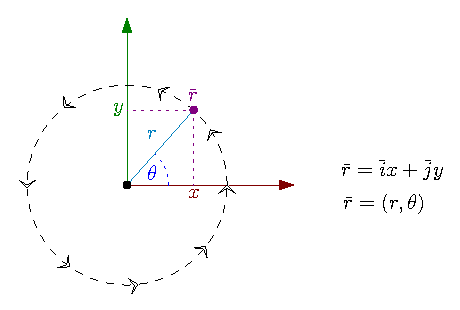
\includegraphics[width=0.5\textwidth]{images/motoCircUn.eps}
    \end{figure} 
\end{center}
Sia $\bar v$ la velocità, essendo il modulo costante, denoteremo $|\bar v|=v_0$. Si considera ora 
la velocità scalare $s$, di cui si ricorda 
$$ \frac{ds}{dt}=v_0$$
Inoltre, sapendo che $\frac{s}{r}=\theta$, si pone 
$$ \frac{ds}{r}=d\theta \implies \frac{ds}{dt}=r\cdot \frac{d\theta}{dt}=v_0$$
Denotiamo $\omega = \dfrac{d\theta}{dt}$, tale termine descrive la variazione dell'angolo nel tempo 
ed è denominato \textbf{velocità angolare}. Il fatto che la velocità dipenda dal raggio $r$, descrive il fatto 
che a parità di velocità angolare, un oggetto che si muove su un cerchio di raggio minore va meno veloce. 
$$ \frac{d\theta}{dt}=\omega \;\;\;\;\;\;\;\;\;\;\;\;\;\;\;
\frac{ds}{dt}=r\omega \;\;\;\;\; \;\;\;\;\;\;\;\;\;\;
v_0=r\omega$$
\end{document}